\documentclass{article}
\usepackage{amsmath}
\usepackage{amssymb}
\usepackage{tikz}
\usetikzlibrary{positioning}

\definecolor {processblue}{cmyk}{0.96, 0, 0, 0}

\begin{document}
	\section{Regular languages}
	\subsection{Deterministic Finite Automaton}
	$\Sigma$ a finite non-empty set called an \textbf{alphabet}. Typically $\Sigma = {0,1}$. \\
	A \textbf{string} $w$ is a finite sequence of symbols -aka. alphabets) in $\Sigma$. \\
	We have:
	\[\epsilon := \text{zero symbols} \]
	\[|w| = \text{number of symbosl in } w \]
	\[\Sigma^{k} := \{ w : w \text{ string over $\Sigma$ } | \; |w| = k \} \]
	\[\Sigma^{\star} := \bigcup_{k \geq 0}{\Sigma^{k}} \text{, } \Sigma^{} := \bigcup_{k \geq 1}{\Sigma^{k}} \]
	A \textbf{language} $L$ over $\Sigma$ is a subset of $\Sigma^{\star}$. The concatenation of $x=x_{1} \dots x_{n}$ and $y=y_{1} \dots y_{m}$ is
	\[ xy = x_{1} \dots x_{n} y_{1} \dots y_{m} \]
	Note : A language is called a \textbf{problem} when strings are given some interpretation (e.g. view $w \in \Sigma^{\star}$ as the binary representation of an integer).
	\par
	An \textbf{automaton} is an abstract model of computation :
	\begin{center}
	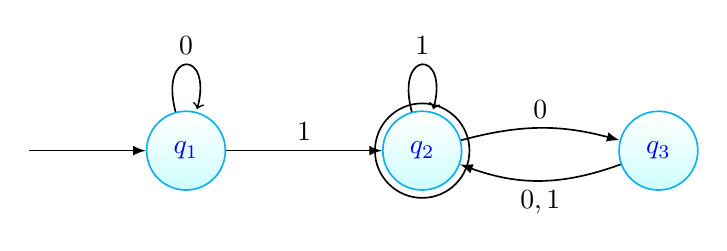
\begin{tikzpicture}[-latex ,auto ,node distance =2 cm and 3cm ,on grid ,
	semithick ,
	state/.style ={ circle ,top color =white , bottom color = processblue!20 ,
		draw,processblue , text=blue , minimum width = 1 cm}]
	\node[state] (A) {$q_{1}$};
	\node[state] (B) [right = of A]{$q_{2}$};
	\node[state] (C) [right = of B]{$q_{3}$};
	\draw[->, >=latex] (-2, 0) to (A); 
	\draw (B) circle(0.6);
	\path (A) edge [loop above] node[above] {$0$} (A);
	\path (A) edge node[above] {$1$} (B);
	\path (B) edge [loop above] node(above) {$1$} (B);
	\path (B) edge [bend left = 15] node(above) {$0$} (C);
	\path (C) edge [bend left = 20] node(below) {$0,1$} (B);
	\end{tikzpicture}
	\end{center}

	Terminology:
	\begin{itemize}
		\item Transition diagram
		\item Start arrow
		\item Accept state
	\end{itemize}

	It reads an input $w=w_{1} \dots w_{n}$ from left to right. It follows the arcs according to the $w_{i}$ starting at the start state. It accepts IFF it ends up in an accepting state after reading the whole input. It rejects otherwise.
	\par 
	Formally, a \textbf{Deterministic Finite Automaton (DFA)} is a 5-tuple $\mathcal{D}=(Q, \sigma, \delta, q_{0}, F)$ where:
	\begin{itemize}
		\item $Q$ is a finite set of states
		\item $\Sigma$ is an alphabet
		\item $\delta : Q \times \Sigma \rightarrow Q$ is a transition function
		\item $q_{0} \in Q$ is the start state
		\item $F \subseteq Q$ is the set of the accepting states
	\end{itemize}
	\par 
	We define the \textbf{Extended Transition Function} $\hat{\delta}$ of $D$ as follows :
	\[ \hat{\delta}(q,\epsilon) := q \text{, } \hat{\delta}(q,xa) := \delta (\hat{\delta}(q,x), a) \]
	We define the \textbf{language of $D$} as follows :
	\[\mathcal{L}(\mathcal{D}) := \{ w \in \Sigma^{\star} \; | \; \hat{\delta}(q_{0}, w) \in F\}\]
	We say that $D$ recognizes a language $L$ if $L = \mathcal{L}(\mathcal{D})$
	We say $L \subseteq \Sigma^{\star}$ is \textbf{regular} if $L=\mathcal{L}(\mathcal{D}) \text{ for some } D$
	
	\subsection{Non-Deterministic Finite Automaton}
	\textbf{Nondeterminism :} A generally useful concept in studying computation. It gives the power of being in several states at once.
	Example:
	\begin{center}
		\begin{tikzpicture}[-latex ,auto ,node distance =2 cm and 3cm ,on grid ,
		semithick ,
		state/.style ={ circle ,top color =white , bottom color = processblue!20 ,
			draw,processblue , text=blue , minimum width = 1 cm}]
		\node[state] (A) {$q_{0}$};
		\node[state] (B) [right = of A] {$q_{1}$};
		\node[state] (c) [right = of B] {$q_{2}$};
		\draw (C) circle(0.6);
		\path (A) edge node[above]{$0$} (B);
		\path (B) edge node[above]{$1$} (C);
		\path (A) [loop above] edge node[above]{$0, 1$} (A);
		\end{tikzpicture}
	\end{center}
	This automaton accepts any string ending in $01$.
	\par 
	Formally : A \textbf{NFA} is a 5-tuple $\mathcal{N} = (Q, \Sigma, \delta, q_{0}, F)$ where $Q, \Sigma,  q_{0}, F$ are defined as previously and $\delta : Q \times \Sigma \rightarrow \mathcal{P}(Q)$ is the transition function.
	\par 
	The extended transition function is:
	\[ \hat{\delta}(q, \epsilon) = \{ q \} \text{, } \hat{\delta}(q, xa) = \bigcup_{p \in \hat{\delta}(q, x)}{\delta(p, a)} \]
	We let:
	\[ \mathcal{L}(\mathcal{N}) = \{ w \in \Sigma^{\star} \; | \; \hat{\delta}(q, xa) \cap F \neq \emptyset \} \]
	
	\subsection{Equivalence of DFAs and NFAs}
	Now, we want to find a way to convert an \textbf{NFA} $\mathcal{N}$ into a \textbf{DFA}, ie. find some $\mathcal{D}$ DFA such that $\mathcal{L}(\mathcal{N}) = \mathcal{L}(\mathcal{D})$ \\
	\textbf{Construction :} \\
	Let $\mathcal{N} = (Q_{\mathcal{N}}, \Sigma, \delta_{\mathcal{N}}, q_{0}, F )$. Consider $\mathcal{D} = (Q_{\mathcal{D}}, \Sigma, \delta_{\mathcal{D}}, q_{0}, F )$ as follows :
	\begin{itemize}
		\item $Q_{\mathcal{D}} = \mathcal{P}(Q_{\mathcal{N}})$
		\item $\delta_{\mathcal{D}}$ so that : $\forall a \in \Sigma, \forall s \in Q_{\mathcal{D}}$, we have :
			\[ \delta_{\mathcal{D}}(s, a) := \bigcup_{p \in S}{\delta_{\mathcal{N}}(p,a)} \]
		\item $F_{\mathcal{D}} = \{ s \subseteq Q_{\mathcal{N}} \; | \; s \cap F_{\mathcal{N}} \neq \emptyset \}$
	\end{itemize}
	\textbf{Theorem :} These automaton denote the same language. $\blacksquare$ \newpage
	\textbf{Note :} When converting, the number of states grows exponentially.
	\subsection{$\mathcal{E}$-NFA}
	\textbf{Idea :} Allow transition without reading any input symbol (ie. reading $\epsilon$). \\
	\textbf{Example :} One can simply build an automaton denoting the union of two regular languages.
	\begin{center}
		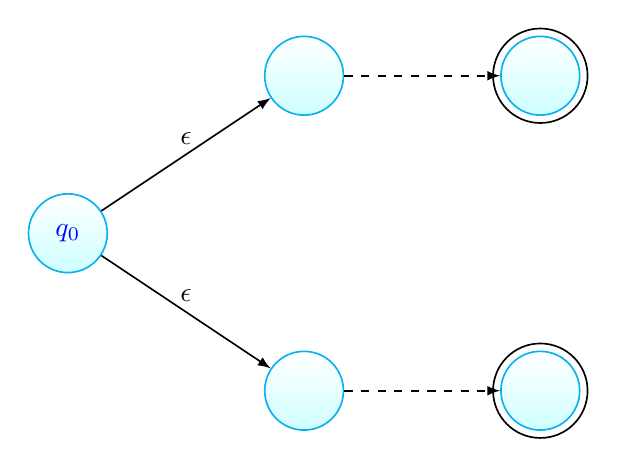
\begin{tikzpicture}[-latex ,auto ,node distance =2 cm and 3cm ,on grid ,
		semithick ,
		state/.style ={ circle ,top color =white , bottom color = processblue!20 ,
			draw,processblue , text=blue , minimum width = 1 cm}]
		\node[state] (A) {$q_{0}$};
		\node[state] (B) [above right = of A] {};
		\node[state] (C) [right = of B] {};
		\node[state] (D) [below right = of A] {};
		\node[state] (E) [right = of D] {};
		\draw (C) circle(0.6);
		\draw (E) circle(0.6);
		\path (A) edge node[above]{$\epsilon$} (B);
		\path (A) edge node[above]{$\epsilon$} (D);
		\draw[dashed] (B) -- (C);
		\draw[dashed] (D) -- (E);
		\end{tikzpicture}
	\end{center}
	\textbf{Definition :} $\mathcal{E}-Closure(q)= \{ q' \in Q \; | \; q'$ can be reached from $q$ by following only $\epsilon$-transitions over multiple transitions\}. We can hence extend the definition of the extended transition function to $\epsilon$-NFAs by having:
	\[ \hat{\delta}(q, \epsilon) := \mathcal{E}-Closure(q) \]
\end{document}













